


% This LaTeX was auto-generated from an M-file by MATLAB.
% To make changes, update the M-file and republish this document.



\documentclass{article}


\usepackage{graphicx}

\usepackage{color}
\usepackage{tabularx}
\usepackage{longtable}
\usepackage{comment}
\usepackage{amsmath}
\usepackage{amssymb}
\usepackage{multirow}
\usepackage{hyperref}
\usepackage{booktabs}
\usepackage{xr}
\usepackage{enumitem}
\usepackage{siunitx}
\usepackage{caption}

\hypersetup{
    bookmarks=true,         % show bookmarks bar?
      colorlinks=true,       % false: boxed links; true: colored links
    linkcolor=red,          % color of internal links (change box
                            % color with linkbordercolor)
    citecolor=green,        % color of links to bibliography
    filecolor=magenta,      % color of file links
    urlcolor=cyan           % color of external links
}

\sloppy
\definecolor{lightgray}{gray}{0.5}


\setlength{\parindent}{0pt}



\begin{document}

    




  
    

\title{Validation Report for Slope Stability Analysis Program}
\author{Henry Frankis}
\date{\today}
\maketitle
\tableofcontents

\section{Introduction}
This document is a report on the results of testing a Slope Stability
Analysis program for validity. The tests are introduced, the results are
displayed, and the meaning of the results are analyzed. Possible further
studies are suggested.




% This LaTeX was auto-generated from an M-file by MATLAB.
% To make changes, update the M-file and republish this document.






  
    

\section{Morgenstern Price Slice Tester} \label{sec:MPTests}
Testing results obtained from the MorgPriceSolver.m program, a module in
the SSA program. Factor of safety results from the program are
compared to results from examples in slope stability papers, to judge the
accuracy of the implemented algorithm. Due to the comparison analysis of
the slip surfaces being imperfect definitive pass or fail assessments are
not used, so results are measured on a relative and objective scale. The
general rule of less relative error between results and comparisons
suggests a more accurate solution can be used. For the same slip the
result may be more accurate towards some comparisons more than others. In
these cases ...?? . As a guideline relative error less than 10\% could be
considered acceptable, less than 5\% good, and less than 1\% excellent.

\subsection{Fredlund and Krahn (1977)}
Results compared to the Fredlund and Krahn (1977) paper. A graph of the
relative error between the factor of safety calculated by the program
with the factor of safety given in the paper, as a function of the number
of analysis slices is used to analyze the results. For this paper a
circular and non circular slip surface for the same slope are studied,
under both dry and wet conditions.


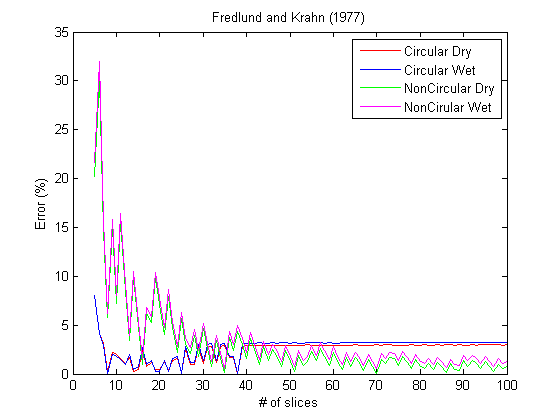
\includegraphics [width=5in]{./VV_SubDocuments/MPSliceTester_01.png}



The figure shows very large error at low numbers of slices, up until
approximately 20 slice analysis. Accuracy then begins to level off and
stays consistent. The graph also shows that the dry analysis has less
relative error than the wet analysis for both circular and non circular
analysis. It can also be seen that the circular slip converges to less
relative error than the non circular analysis. This suggests that the
simpler dry and circular cases produce more accurate results, however
further analysis of this type would be needed for a concrete conclusion.

~\newline \noindent
Inspecting the computation of the factor of safety at extremely large
numbers of slices shows no noticeable change in the returned value.
Convergence to the same factor of safety occurs at 100 and 100000
slices, as seen on the following graph.


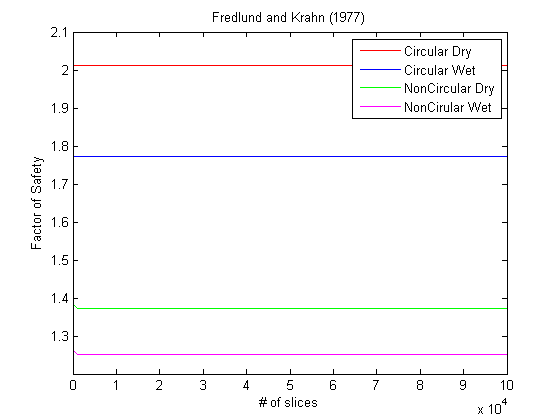
\includegraphics [width=5in]{./VV_SubDocuments/MPSliceTester_02.png}



The next graph shows the change in computation time for calculation of
the slope with different slice numbers. An approximately linear increase
in computation time with number of analysis slices can be seen. As using
a large number of slices sees no noticeable increase in the calculation
of the Factor of Safety, the increased computation time makes using more
slices than approximately 50 unnecessary. When compared to the 
computation time results the RFEM solver (\ref{sec:RFEMTests}), it can be 
seen that the computation time for the morgenstern price algorithm is 
significantly less.


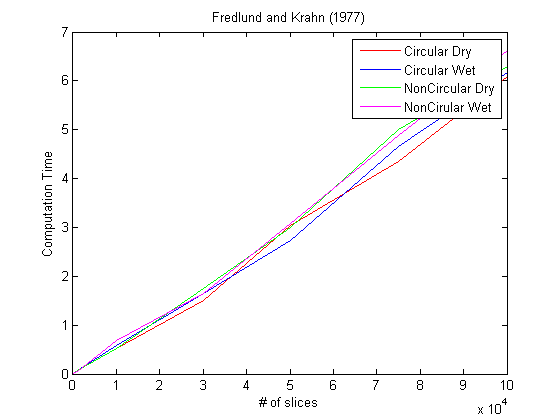
\includegraphics [width=5in]{./VV_SubDocuments/MPSliceTester_03.png}



\subsection{Examples 1 - 5}
Results from the examples used in the papers: Greco (1996), Malkawi et al
(2001) Zolfaghari et al (2005), Sarma and Tan (2006), Pham and Fredlund
(2003), Cheng et al (2007), and Li et al (2010). Results followed the
same general pattern as the previous test: Converging to a consistent
factor of safety at approximately 25 slices. Relative error between
results achieved and the results from the examples in the papers are all
less than 10\%, and for some lower than 1\%. For examples with multiple
comparisons the result usually converges very strongly to at least one
of the comparisons. It should again be noted that the accuracy of results
is relative only to the accuracy of the results from the comparison
papers. However consistently high accuracy compared to results from
different papers in many different examples, means a large true error
would suggest a flaw in the slope stability analysis community as a
whole. Not displayed here, but it was also seen that a large number of
slices resulted in no noticeable change in the factor of safety
calculation.


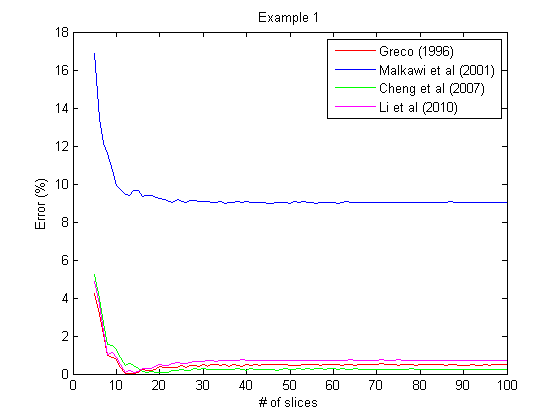
\includegraphics [width=5in]{./VV_SubDocuments/MPSliceTester_04.png}




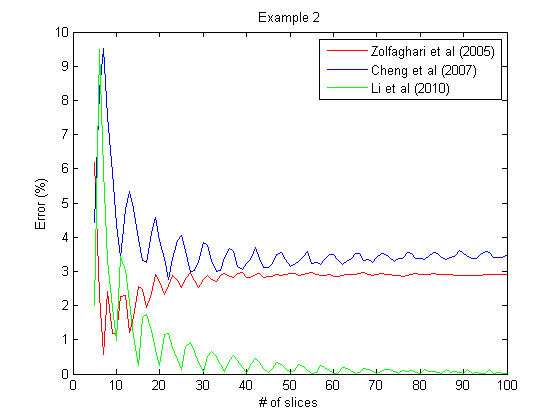
\includegraphics [width=5in]{./VV_SubDocuments/MPSliceTester_05.png}




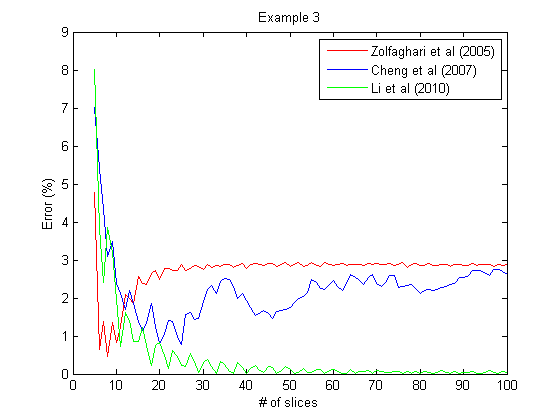
\includegraphics [width=5in]{./VV_SubDocuments/MPSliceTester_06.png}




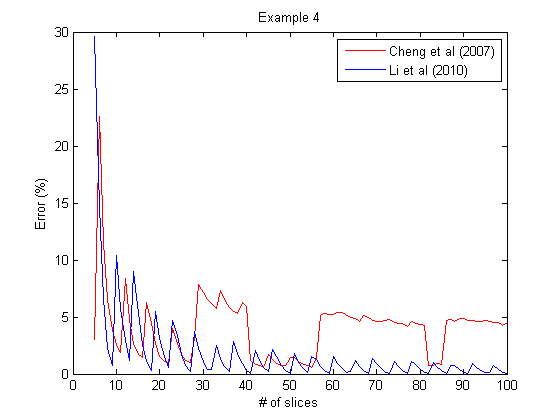
\includegraphics [width=5in]{./VV_SubDocuments/MPSliceTester_07.png}




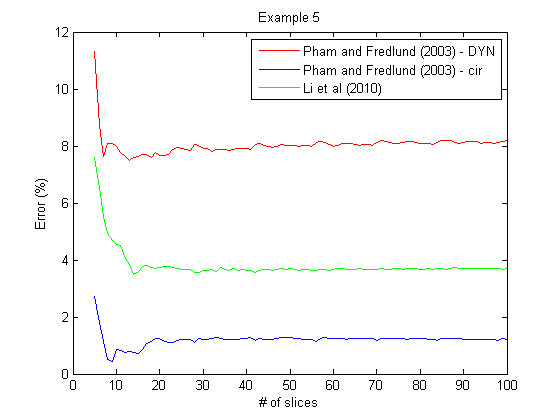
\includegraphics [width=5in]{./VV_SubDocuments/MPSliceTester_08.png}



\subsection{Example 6}
Results from the example used in the papers: Pham and Fredlund (2003), Li
et al (2010). Analysis of this example demonstrated non convergence of
the Factor of Safety calculation for specific slice counts of the
circular Pham and Fredlund analysis. Non convergence occurs when the
algorithm calculates a very low factor of safety, or if the algorithm
solution doesn't become consistent within the limited amount of
iterations.


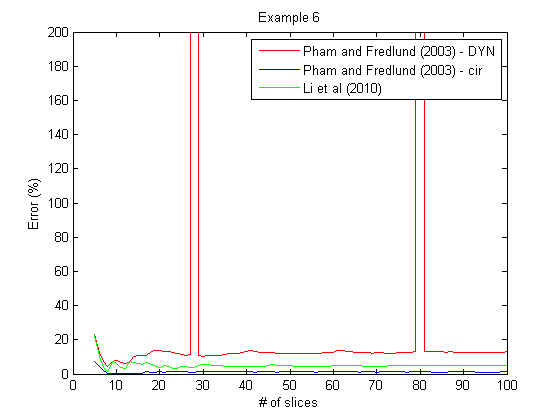
\includegraphics [width=5in]{./VV_SubDocuments/MPSliceTester_09.png}



As a special case the limiting number of iterations allowed for the
analysis was raised from 20 iterations to 30. The previously non
converging results now converge to approximately 15% error, as can be
seen in the following figure. This is less accurate than the results seen
previously, which were generally under 10%. This demonstrates the trade
off between raising the iteration limit allowing better convergence, but
decreasing the overall accuracy of the solver.

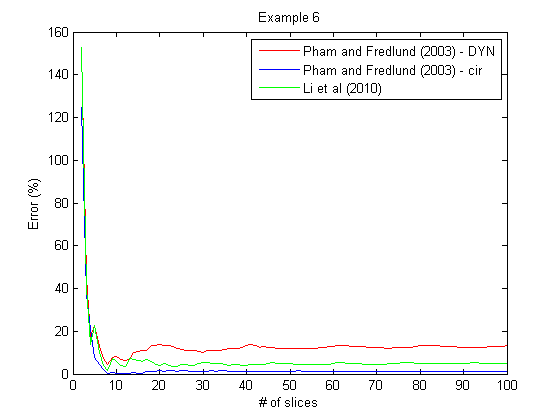
\includegraphics[width=5in]{./VV_SubDocuments/MPSlice_SpecialCase.png}





% This LaTeX was auto-generated from an M-file by MATLAB.
% To make changes, update the M-file and republish this document.






  
    

\section{RFEM Slice Tester} \label{sec:RFEMTests}
Testing results obtained from the RFEMSolver.m program, a module in
the SSA program. Factor of safety results from the program are
compared to results from examples in slope stability papers, to judge the
accuracy of the implemented algorithm. As seen mentioned in the
Morgenstern Price solver testing (section \ref{sec:MPTests}), due to the
imperfect nature of the comparisons, results are judged on a relative
basis. Example numbers refer to the same slope/slip problem as
analyzed in the Morgenstern Price tests. The comparisons from scientific
papers were performed using non RFEM solver algorithms, such as
Morgenstern Price or Spencer's method. Therefore the relative accuracy of
the implemented Morgenstern Price algorithm may appear higher, this does
not also suggest the Morgenstern Price solver is truly more accurate
however. Ideally and as is seen the RFEM solver should converge to a
solution similar to the comparison slip, as two different methods
calculating similar answers suggest accuracy of both methods.

\subsection{Example 1}
Results compared to those from Greco (1996), Malwaki et al (2001),
Cheng et al(2007), and Li et al (2010). A graph of the relative error
between the factor of safety calculated by the program with the factor of
safety given in the papers is used to analyze the results. The results
using the Morgenstern Price algorithm is also plotted. As the comparison
was also performed using the Morgenstern Price algorithm this relative
error is almost 0.


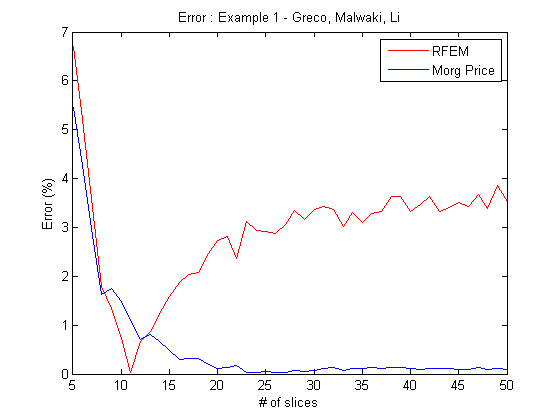
\includegraphics [width=5in]{./VV_SubDocuments/RFEMSliceTester_01.png}



The figure shows convergence to a consistent relative error of less than
5\% after approximately 25 slices for the RFEM solver. This is a positive
result suggesting accuracy of both methods. However as seen in the
following figure the RFEM algorithm requires significantly more
computation time than the Morgenstern Price algorithm (section
\ref{sec:MPTests}). The large difference in calculation time makes the
Morgenstern Price solver much more efficient, especially when performing
repeated analysis in the Genetic Algorithm search.


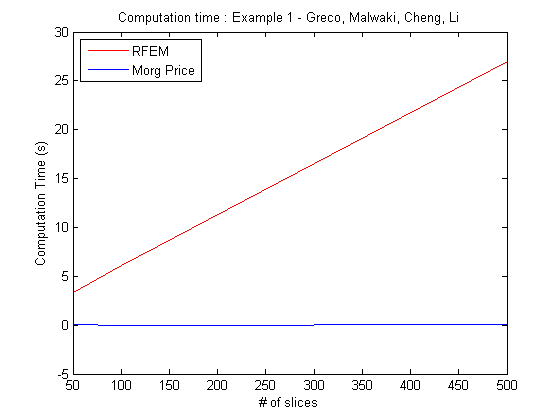
\includegraphics [width=5in]{./VV_SubDocuments/RFEMSliceTester_02.png}



\subsection{Examples 2 and 6}
Results compared to those from Zolfaghari et al (2005), Cheng et al
(2007), Li et al (2010) and Pham and Fredlund (2003). The graphs of these
examples continue to show convergence to relative error of approximately
5\% - 10\% after approximately 25 steps. Again these are all positive
results suggesting accuracy of both solvers.


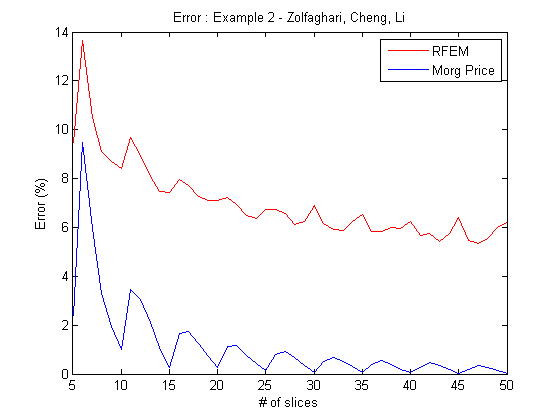
\includegraphics [width=5in]{./VV_SubDocuments/RFEMSliceTester_03.png}




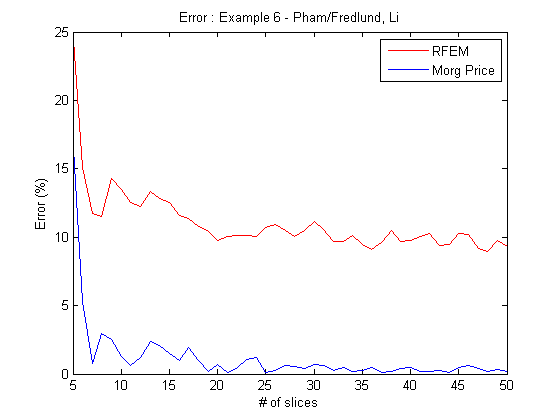
\includegraphics [width=5in]{./VV_SubDocuments/RFEMSliceTester_04.png}







% This LaTeX was auto-generated from an M-file by MATLAB.
% To make changes, update the M-file and republish this document.






  
    

\section{Genetic Algorithm Tester} \label{sec:GenAlgTests}
This script file tests the function GenAlg.m program, a module in the SSA
program. The program will be tested for the relative error of the
critical factor of safety for an example slip compared to the critical
factor of safety from a paper analyzing the same example slip. Repeated
analysis of an example slip will also be performed to analyze the
consistency of the algorithm.

\subsection{Example 1}
Comparing results for the example from Greco (1996), Malkawi et al
(2001), Cheng et al (2007), Li et al (2010).

\subsubsection{Consistency Testing}
Firstly this example is used as a method of testing the consistency of
the implemented genetic algorithm. Using the same input for the genetic
algorithm to solve for the critical slip surface 15 times the physical
and critical factor of safety range the algorithm generates as critical
clip surfaces will be investigated.

For each solution a second order polynomial is fit to the vertexes
describing that solutions critical slip surface. The approximately
quadratic shape of the slip surface makes a second order polynomial an
appropriate fit. Solutions are of the form:
\[ y(x) = C_{\text{1}} \cdot x^2 + C_{\text{2}} \cdot x + C_{\text{3}} \]
Where $y$ is the vertical height of the slip surface at horizontal point
$x$. The following histograms show the spread of the fitting constants
$C_\text{1}$, $C_\text{2}$, and $C_\text{3}$. If the algorithm is
consistent the slip surfaces will follow similar shapes and the
constants will have little spread.


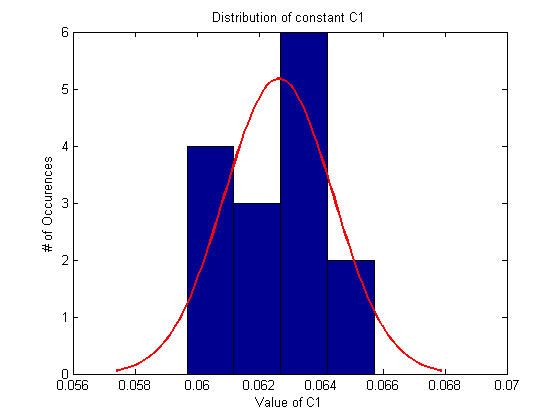
\includegraphics [width=5in]{./VV_SubDocuments/GenAlgTester_01.png}




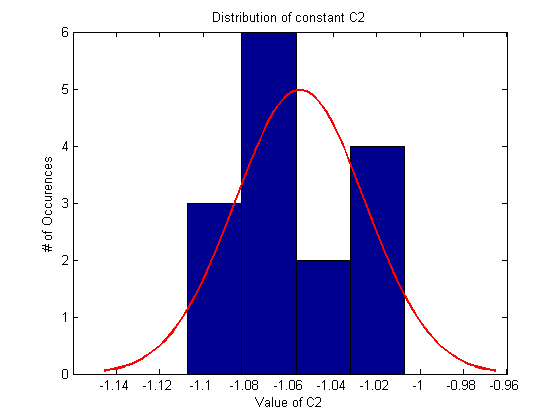
\includegraphics [width=5in]{./VV_SubDocuments/GenAlgTester_02.png}




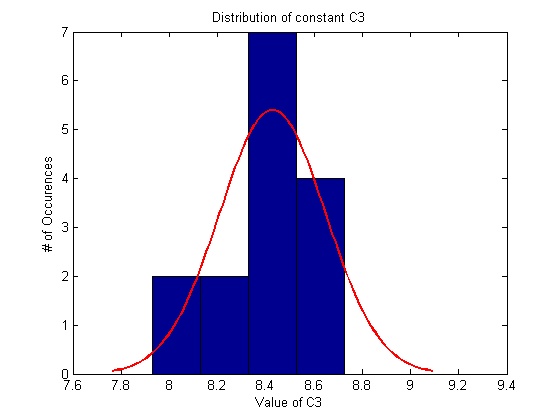
\includegraphics [width=5in]{./VV_SubDocuments/GenAlgTester_03.png}



The results in the figures show that the normal distribution of results
is approximately followed with few outlying data points, and that the
spread of the constants for the different fits is small, differing over a
small range. This suggests a consistent solution.

        
\color{lightgray} \begin{verbatim}
C1 has a standard deviation of 0.00
C2 has a standard deviation of 0.03
C3 has a standard deviation of 0.22
\end{verbatim} \color{black}
    

The next figure shows a plot of all the critical slip surfaces generated,
supporting the previous findings by showing all the slip surfaces
existing along a narrow band. The band width was measured at the entry
and exit points of the slope for context.

        
\color{lightgray} \begin{verbatim}
The entry band width was : 0.837
The exit band width was : 1.692

\end{verbatim} \color{black}
    


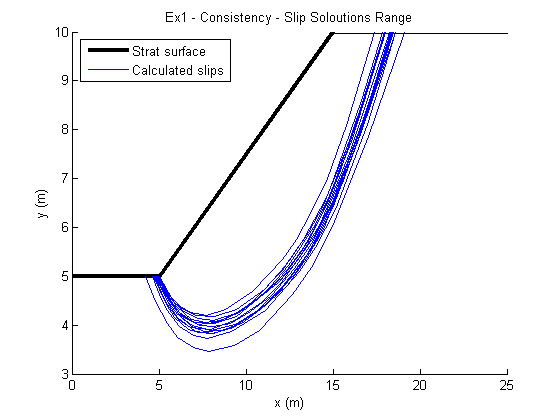
\includegraphics [width=5in]{./VV_SubDocuments/GenAlgTester_04.png}



The previous results demonstrate that the algorithm generates spatially
consistent solutions. The consistency of the Factor of Safety for the
critical slips surface will now be investigated.  The following histogram
summarizes the distribution of calculated critical factors of safety. The
figure shows a consistent factor of safety calculation, with results
differing over a small range.

        
\color{lightgray} \begin{verbatim}
The average critical slip Factor of Safety 
 is FS=1.3157, with a standard deviation 
 of 0.0036, and a minimum of FS=1.3124
\end{verbatim} \color{black}
    


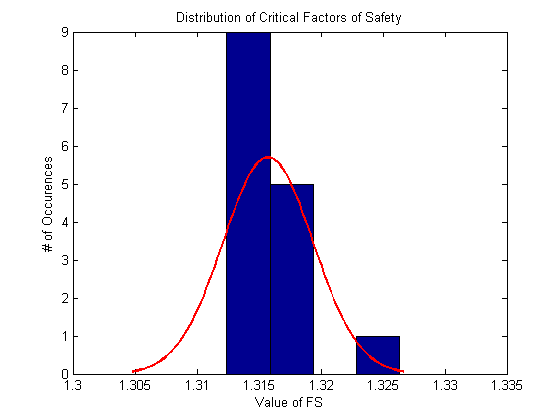
\includegraphics [width=5in]{./VV_SubDocuments/GenAlgTester_05.png}



The following figure shows the progression of the critical slip factor of
safety over each generation of the genetic algorithm. The red dot
represents the final generation. The figure generally shows convergence
after approximately 130 generations. All solutions also seem to follow
the same general path to convergence.

        
\color{lightgray} \begin{verbatim}
The average number of generations for convergence is 134
 The maximum is 319, and the minimum is 102
 The standard deviation of all trials is 55
\end{verbatim} \color{black}
    


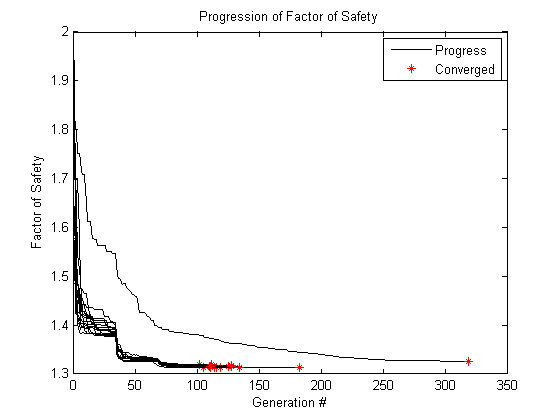
\includegraphics [width=5in]{./VV_SubDocuments/GenAlgTester_06.png}



The results seen in this section all suggest that the genetic algorithm
can consistently converge to a common critical slip, with a common
critical factor of safety.

\subsubsection{Error Test}
The Example 1 slope problem will now be measured for accuracy based on
the difference between results generated by the algorithm, and results
found scientific papers that analyzed the same example slope. A
comparison between the slip surfaces and factors of safety is made. For
this example the average of all generated slip surfaces was used.
\newline\newline\noindent
The accuracy of the slip is shown visually with a plot, and also
measured using a \textit{distance error} metric. The metric slices the
calculated slip surface, and comparison slip surface equally into 10
description vertexes. The average of distance between vertexes of the
same indice, is then considered the \textit{distance error}.
\newline\newline\noindent
The accuracy of the factor of safety is measured based on relative error
with the comparison factor of safety.

        
\color{lightgray} \begin{verbatim}
Example 1 - Slip
Author                    entry x       exit x    distance error
Calculated                 4.8225      18.2362
Greco (1996)               4.8077      18.2911          2.3715
Malkawi et al (2001)       3.5400      20.1419         10.0779
Cheng et al (2007)         4.5258      18.3943          2.9385
Li et al (2010)            4.6000      18.5300          2.7468

Example 1 - Factor of Safety
Author                         Fs     err (%)      time
Calculated                 1.3157               18.9853
Greco (1996)               1.3270      0.8494
Malkawi et al (2001)       1.2380      6.2786
Cheng et al (2007)         1.3250      0.6997
Li et al (2010)            1.3270      0.8494
\end{verbatim} \color{black}
    


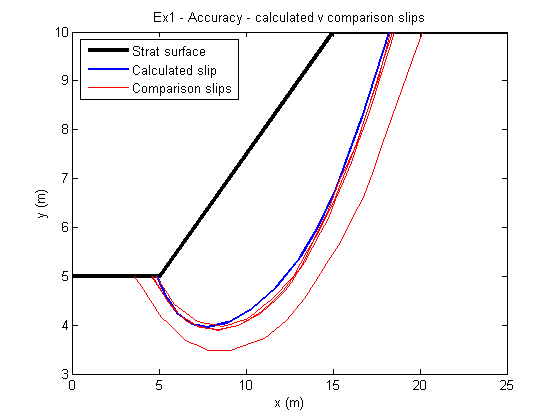
\includegraphics [width=5in]{./VV_SubDocuments/GenAlgTester_07.png}



\subsection{Examples 2-7}
Examples 2-7 compare critical factor of safety results for the program to
the results of many different papers. The tables show that results are
very accurate compared to the results in the paper, with a relative
factor of safety errors generally less than 5\% for at least one of the
comparison slips. The plots of the slip surfaces also show a critical
slip that is reasonably similar to the comparison slips.
\newline\newline\noindent
The only exception comes in Example 6. Approximately half the time a
critical factor of safety equal to the result in the paper will be
calculated, while the other half a factor of safety of approximately 0.6
will be calculated. Further investigation of this is found in
\ref{sec:Ex6Tests}.

\subsubsection*{Example 2}
\textbf{Papers:} Zolfaghari et al (2005), Cheng et al (2007),
Li et al (2010)

        
\color{lightgray} \begin{verbatim}
Example 2 - Slip
Author                    entry x       exit x    distance error
Calculated                12.6982      30.5063
Zolfaghari et al (2005)   13.0126      30.6803          0.1271
Cheng et al (2007)        12.2707      31.0044          0.1077
Li et al (2010)           12.6800      30.5300          0.0091

Example 2 - Factor of Safety
Author                         Fs     err (%)      time
Calculated                 1.1095               16.5205
Zolfaghari et al (2005)    1.2400     10.5203
Cheng et al (2007)         1.1010      0.7765
Li et al (2010)            1.1130      0.3101
\end{verbatim} \color{black}
    


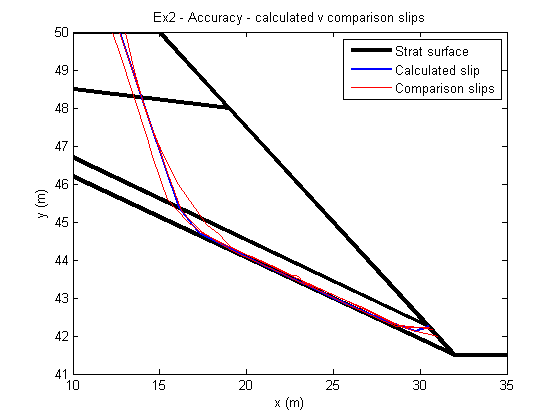
\includegraphics [width=5in]{./VV_SubDocuments/GenAlgTester_08.png}



\subsubsection*{Example 3}
\textbf{Papers:} Zolfaghari et al (2005), Cheng et al (2007),
Li et al (2010)

        
\color{lightgray} \begin{verbatim}
Example 3 - Slip
Author                    entry x       exit x    distance error
Calculated                12.5196      26.6608
Zolfaghari et al (2005)   14.4928      26.2681          0.3857
Cheng et al (2007)        12.0100      26.9014          0.1146
Li et al (2010)           12.5800      26.9200          0.0672

Example 3 - Factor of Safety
Author                         Fs     err (%)      time
Calculated                 1.3334               26.4734
Zolfaghari et al (2005)    1.4800      9.9039
Cheng et al (2007)         1.3490      1.1548
Li et al (2010)            1.3350      0.1182
\end{verbatim} \color{black}
    


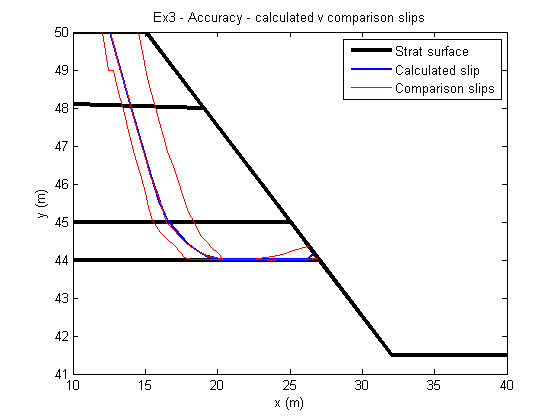
\includegraphics [width=5in]{./VV_SubDocuments/GenAlgTester_09.png}



\subsubsection*{Example 4}
\textbf{Papers:} Cheng et al (2007), Li et al (2010)

        
\color{lightgray} \begin{verbatim}
Example 4 - Slip
Author                    entry x       exit x    distance error
Calculated                13.2859      29.2819
Cheng et al (2007)        12.0749      31.9000          0.4879
Li et al (2010)           12.6500      31.9100          0.4900

Example 4 - Factor of Safety
Author                         Fs     err (%)      time
Calculated                 1.3275               26.8166
Cheng et al (2007)         1.1840     12.1204
Li et al (2010)            1.1970     10.9027
\end{verbatim} \color{black}
    


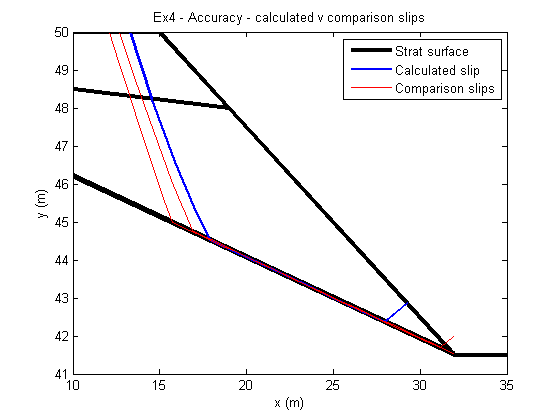
\includegraphics [width=5in]{./VV_SubDocuments/GenAlgTester_10.png}



\subsubsection*{Example 5}
\textbf{Papers:} Pham and Fredlund (2003), Li et al (2010)

        
\color{lightgray} \begin{verbatim}
Example 5 - Slip
Author                    entry x       exit x    distance err
Calculated                16.1920      40.1603
Pham and Fredlund (2003)  15.9700      43.9000          1.7744
Li et al (2010)           15.4100      41.8900          0.8691

Example 5 - factor of Safety
Author                         Fs     err (%)      time
Calculated                 1.4317               19.3441
Pham and Fredlund (2003)   1.4130      1.3233
Li et al (2010)            1.4080      1.6831
\end{verbatim} \color{black}
    


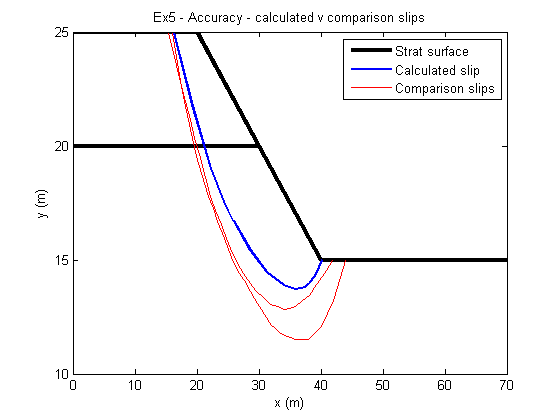
\includegraphics [width=5in]{./VV_SubDocuments/GenAlgTester_11.png}



\subsubsection*{Example 6}
\textbf{Papers:} Pham and Fredlund (2003), Li et al (2010)

        
\color{lightgray} \begin{verbatim}
Example 6 - Slip
Author                    entry x       exit x    distance error
Calculated                17.5144      44.7286
Pham and Fredlund (2003)  14.0000      47.9868          1.1717
Li et al (2010)           13.9200      49.1400          1.3511

Example 6 - Factor of Safety
Author                         Fs     err (%)      time
Calculated                 0.5215               19.0789
Pham and Fredlund (2003)   1.0000     47.8494
Li et al (2010)            1.0170     48.7212
\end{verbatim} \color{black}
    


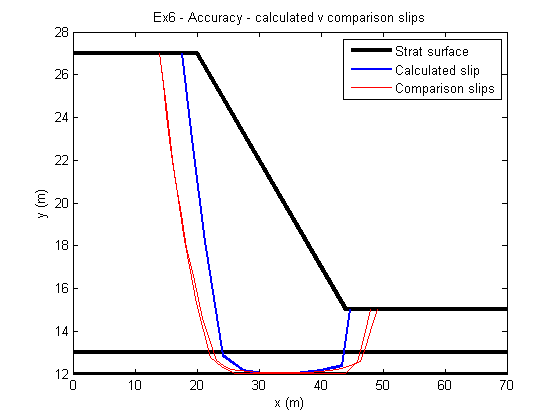
\includegraphics [width=5in]{./VV_SubDocuments/GenAlgTester_12.png}



\subsubsection*{Example 7}
\textbf{Papers:} Fredlund and Krahn (1977)

        
\color{lightgray} \begin{verbatim}
Example 7 - Slip
Author                    entry x       exit x    distance error
Calculated                12.5593      43.5584
Fredlund and Krahn (1977) 13.9714      48.3809          1.6641

Example 7 - Factor of Safety
Author                         Fs     err (%)      time
Calculated                 1.1398               18.0649
Fredlund and Krahn (1977)  1.2450      8.4466
\end{verbatim} \color{black}
    


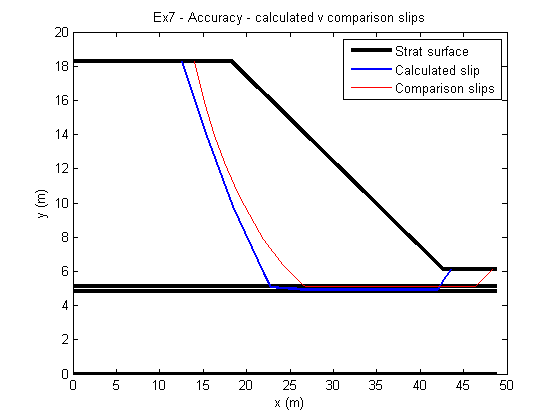
\includegraphics [width=5in]{./VV_SubDocuments/GenAlgTester_13.png}







% This LaTeX was auto-generated from an M-file by MATLAB.
% To make changes, update the M-file and republish this document.






  
    

\section{Kinematic Admissibility Tester} \label{sec:KinTests}
Testing results obtained from the KinAdm.m program, a
module in the Slope Stability Analysis program. The tester will test the
algorithm to ensure it can correctly identify when a slip surface fails
the 6 failure criterion.

\subsection{Testing}
The module will now be tested for the different failure criterion. A
kinematically inadmissible test will return a value pass=0, and a failure
code detailing the cause of the failure. All other values should return a
value pass=1. All failure criteria will pass boundary cases. The failure
criterion are tested individually with a simple slope surface, and slip
surfaces designed to test the failure. Each failure test will give a slip
designed to pass, a boundary case, and one designed to fail.

\subsubsection*{Failure (i)}
The first criteria of a kinematically admissible surface is that the
x-ordinates of the input slip surface vertexes do not decrease when
reading the list of vertexes from beginning to end. (A) is a test with
constantly increasing x-ordinates. (B) is a test case with equivalent
x-ordinates. (C) is a case with decreasing x-ordinates. Results follow:

        
\color{lightgray} \begin{verbatim}
Failure (i):
(A): pass=1
(B): pass=1
(C): pass=0 Failure Code1 - Non monotonic x
\end{verbatim} \color{black}
    

\subsubsection*{End Adjustments}
The second criteria of a kinematically admissible surface is that the
start and end vertexes of the slip surface match the y-ordinate of the
uppermost stratigraphic layer at the specified x-ordinate.
The module will not fail the slip surface, but will adjust the y value of
the end vertexes. (A) is a test with vertexes above the uppermost
stratigraphic layer. (B) is a test with vertexes on the uppermost
stratigraphic layer. (C) is a test with vertexes below the uppermost
stratigraphic layer. Vertice adjustment refers to the y values of the
vertexes.

        
\color{lightgray} \begin{verbatim}
End Adjustments:
(A): pass=1, Start vertice adjustment,21->20 End vertice adjustment,13->12
(B): pass=1, Start vertice adjustment,20->20 End vertice adjustment,12->12
(C): pass=1, Start vertice adjustment,19->20 End vertice adjustment,11->12
\end{verbatim} \color{black}
    

\subsubsection*{Failure (ii)}
The vertexes of the slip surface must be within the specified x-ordinate
range of the uppermost stratigraphic layer. (A) is a test case with
vertexes that stay within the uppermost stratigraphic layers range. (B)
is a test with a vertice x-ordinate that goes below the minimum range of
the uppermost stratigraphic layer. (C) is a test with a vertice
x-ordinate that goes above the maximum range of the uppermost
stratigraphic layer.

        
\color{lightgray} \begin{verbatim}
Failure (ii):
(A): pass=1
(B): pass=0 Failure Code2 - Vertex outside x range
(C): pass=0 Failure Code2 - Vertex outside x range
\end{verbatim} \color{black}
    

\subsubsection*{Failure (iii)}
The non end vertexes of the slip surface must be below the uppermost
stratigraphic layer. End vertexes will be moved onto the uppermost
stratigraphic layer, and therefore don't interact with this case. This
failure case checks only vertexes, line segments above the uppermost
strat are checked in failure (iv). (A) is a test with vertexes below the
uppermost stratigraphic layer. (B) is a test with vertexes on the
uppermost stratigraphic layer. (C) is a test with the first interior
vertice above the uppermost stratigraphic layer. (D) is a test with the
last interior vertice above the uppermost stratigraphic layer of the slip
surface.

        
\color{lightgray} \begin{verbatim}
Failure (iii):
(A): pass=1
(B): pass=1
(C): pass=0 Failure Code3 - Vertex above surface
(D): pass=0 Failure Code3 - Vertex above surface
\end{verbatim} \color{black}
    

\subsubsection*{Failure (iv)}
Line segments between vertexes of the slip surface cannot go above the
uppermost stratigraphic layer. (A) is a test with all line segments below
the uppermost stratigraphic surface. (B) is a test case with a line
segment on the uppermost stratigraphic layer. (C) is a test case with a
line segment below the uppermost stratigraphic layer. the test is
performed on the three interior line segments of the uppermost
stratigraphic layer, going from slip entrance to exit as Strat Line
Segments 1,2,3.

        
\color{lightgray} \begin{verbatim}
Failure (iv) Strat Line Segment 1:
(A): pass=1
(B): pass=1
(C): pass=0 Failure Code4 - Surface Intersection

Failure (iv) Strat Line Segment 2:
(A): pass=1
(B): pass=1
(C): pass=0 Failure Code4 - Surface Intersection

Failure (iv) Strat Line Segment 3:
(A): pass=1
(B): pass=1
(C): pass=0 Failure Code4 - Surface Intersection
\end{verbatim} \color{black}
    

\subsubsection*{Failure (v)}
The slip surface must be concave upwards. The slope of line segments
between vertexes of the slip surface must go from a large magnitude
negative number towards a large magnitude positive number when connecting
vertexes from slip entrance to exit. (A) test a case where slip surface
slopes are increasing. (B) tests a case where slip surface
slopes are constant. (C) tests a case where slip slopes experience a
decrease.

        
\color{lightgray} \begin{verbatim}
Failure (v):
(A): pass=1
(B): pass=1
(C): pass=0 Failure Code5 - Concave Down, mcur=-1.02 mprv=-0.98
\end{verbatim} \color{black}
    

\subsubsection*{Failure (vi)}
Slip surfaces cannot have angles less than 110 degrees (1.9199 rads)
between adjacent line segments connecting vertexes. (A) tests a case with
a greater than 110 degree slope. (B) tests a case with an exactly 110
degree slope. (C) tests a case with a less than 110 degree slope.

        
\color{lightgray} \begin{verbatim}
Failure (vi):
(A): pass=0 Failure Code6 - Sharp angle, Theta=1.9078
(B): pass=0 Failure Code6 - Sharp angle, Theta=1.9003
(C): pass=0 Failure Code6 - Sharp angle, Theta=1.8929
\end{verbatim} \color{black}
    

The results seen differ slightly from whats expected, with all cases
failing reporting angles just below the 1.9199 rad cut off, despite case
(A) being greater than this angle, and (B) being approximately
equivalent, based on geometric analysis. The minor error in angle
calculation likely comes from a \textit{pi} rounding error. Other than
this small error, all other tests were successful.





% This LaTeX was auto-generated from an M-file by MATLAB.
% To make changes, update the M-file and republish this document.






  
    

\section{Input Tester} \label{sec:InputTests}
Testing results obtained for the Input.m program a module in the Slope
Stability Analysis program. Tested using the SSA\_InputTester.m script.
Tests used the script SSA\_InputSpecial.m in place of Input.m, where
SSA\_InputSpecial is identical with the exception of predetermined command
line inputs. The tester will test the algorithm to ensure it can
correctly identify faulty input files, through various failure
mechanisms.

\renewcommand*{\arraystretch}{1.5}
\begin{longtable}{| m{0.3\textwidth} | m{0.25\textwidth} |
m{0.45\textwidth} |} \hline
\textbf{Error Type} & \textbf{Case} & \textbf{Error Code}
\\ \hline

good file & / &

\\ \hline

\multirow{2}{0.3\textwidth} {Dimensions \\ - input file incorrectly
identifies the number of stratigraphic layers describing the slope} &
understate &

        
\color{lightgray} 
Input Error : Expected 1 and  detected 2 stratigraphic layers
 \color{black}
    

\\ \cline{2-3} & overstate &

        
\color{lightgray} 
Input Error : Expected 3 and  detected 2 stratigraphic layers
 \color{black}
    

\\ \hline

\multirow{2}{0.3\textwidth} {Dimensions \\ - input file incorrectly
identifies the number of vertexes describing a soil layer} & understate &

        
\color{lightgray} 
Input Error : Expected 4 and detected 5 vertex sets describing stratigraphic layer 1
 \color{black}
    

\\ \cline{2-3} & overstate &

        
\color{lightgray} 
Input Error : Expected 6 and detected 5 vertex sets describing stratigraphic layer 1
 \color{black}
    

\\ \hline

\multirow{2}{0.3\textwidth} {Dimensions \\ - input file incorrectly gives
the number of soil properties necessary to describe a layer} & missing
properties &

        
\color{lightgray} 
Input Error : Stratigraphic soil properties not fully defined
 \color{black}
    

\\ \cline{2-3} & extra properties &

        
\color{lightgray} 
Input Error : An extra soil data input has been given
 \color{black}
    

\\ \hline

\multirow{2}{0.3\textwidth} {Analysis \\ - input files given soil motion
direction does not match the geometry of the slope} & left to right &

        
\color{lightgray} 
Input Error : Detected soil motion direction (left to right), does not match given soil motion
 \color{black}
    

\\ \cline{2-3} & right to left &

        
\color{lightgray} 
Input Error : Detected soil motion direction (right to left), does not match given soil motion
 \color{black}
    

\\ \hline

\multirow{2}{0.3\textwidth} {Analysis \\ - input files given vertices of
a soil layer or piezometric surface not ordered in terms of increasing
x-ordinates.} & soil layer &

        
\color{lightgray} 
Input Error : Given x-ordinates describing layer 2 are not in an increasing order
 \color{black}
    

\\ \cline{2-3} & piezometric surface &

        
\color{lightgray} 
Input Error : Given initial x-ordinate of 0.0, and final x-ordinate of 75.0, of layer 2, do not match those given in the first layer with an initial x of 0.0 and final x of 70.0
 \color{black}
    

\\ \hline

\multirow{4}{0.3\textwidth} {Analysis \\ - input file gives end vertexes
of a soil layer that does not match the end x-ordinate range of the
uppermost stratigraphic layer.} & end vertice \newline - high &

        
\color{lightgray} 
Input Error : Given initial x-ordinate of 0.0, and final x-ordinate of 75.0, of layer 2, do not match those given in the first layer with an initial x of 0.0 and final x of 70.0
 \color{black}
    

\\ \cline{2-3} & end vertice \newline - low &

        
\color{lightgray} 
Input Error : Given initial x-ordinate of 0.0, and final x-ordinate of 60.0, of layer 2, do not match those given in the first layer with an initial x of 0.0 and final x of 70.0
 \color{black}
    

\\ \cline{2-3} & start vertice \newline - high &

        
\color{lightgray} 
Input Error : Given initial x-ordinate of 5.0, and final x-ordinate of 70.0, of layer 2, do not match those given in the first layer with an initial x of 0.0 and final x of 70.0
 \color{black}
    

\\ \cline{2-3} & start vertice \newline - low &

        
\color{lightgray} 
Input Error : Given initial x-ordinate of -5.0, and final x-ordinate of 70.0, of layer 2, do not match those given in the first layer with an initial x of 0.0 and final x of 70.0
 \color{black}
    

\\ \hline

\multirow{4}{0.3\textwidth} {Analysis \\ - input file gives end vertexes
of a piezometric surface that does not match the end x-ordinate range of
the uppermost stratigraphic layer.} & end vertice \newline - high &

        
\color{lightgray} 
Input Error : Given initial x-ordinate of 0.0, and final x-ordinate of 75.0, of the piezometric surface, do not match those given in the first layer with an initial x of 0.0 and final x of 70.0
 \color{black}
    

\\ \cline{2-3} & end vertice \newline - low &

        
\color{lightgray} 
Input Error : Given initial x-ordinate of 0.0, and final x-ordinate of 65.0, of the piezometric surface, do not match those given in the first layer with an initial x of 0.0 and final x of 70.0
 \color{black}
    

\\ \cline{2-3} & start vertice \newline - high &

        
\color{lightgray} 
Input Error : Given initial x-ordinate of 10.0, and final x-ordinate of 70.0, of the piezometric surface, do not match those given in the first layer with an initial x of 0.0 and final x of 70.0
 \color{black}
    

\\ \cline{2-3} & start vertice \newline - low &

        
\color{lightgray} 
Input Error : Given initial x-ordinate of -10.0, and final x-ordinate of 70.0, of the piezometric surface, do not match those given in the first layer with an initial x of 0.0 and final x of 70.0
 \color{black}
    

\\ \hline

\multirow{2}{0.3\textwidth} {Constraints \\ - The effective angle of
friction given for all soil layers must be between 0 and 90 degrees.} &
$> 90$ &

        
\color{lightgray} 
Input Error : Effective angle of friction of layer 1 does not meet physical constraints, must be between 0 and 90 degrees, given 100.0
 \color{black}
    

\\ \cline{2-3} & $< 90$ &

        
\color{lightgray} 
Input Error : Effective angle of friction of layer 1 does not meet physical constraints, must be between 0 and 90 degrees, given -10.0
 \color{black}
    

\\ \hline

Constraints \newline - The cohesion given for all soil layers must be
greater than 0. & $< 0$ &

        
\color{lightgray} 
Input Error : cohesion of layer 1 does not meet physical constraints, must be greater than 0, given -5.0
 \color{black}
    

\\ \hline

Constraints \newline - The soil weight given for all soil layers must be
greater than 0. & $< 0$ &

        
\color{lightgray} 
Input Error : Soil weight of layer 1 does not meet physical constraints, must be greater than 0, given -15.0
 \color{black}
    

\\ \hline

Constraints \newline - The saturated soil weight given for all soil
layers must be greater than 0. & $< 0$ &

        
\color{lightgray} 
Input Error : Saturated soil weight of layer 1 does not meet physical constraints, must be greater than 0, given -15.0
 \color{black}
    

\\ \hline

\multirow{2}{0.3\textwidth} {Constraints \\ - The poisson's ratio
given for all soil layers must be between 0 and 90 degrees.} &
$> 1$ &

        
\color{lightgray} 
Input Error : Given initial x-ordinate of 0.0, and final x-ordinate of 75.0, of layer 2, do not match those given in the first layer with an initial x of 0.0 and final x of 70.0
 \color{black}
    

\\ \cline{2-3} & $< 0$ &

        
\color{lightgray} 
Input Error : Poissons ratio of layer 1 does not meet physical constraints, must be greater than 0 and less than 1, given -0.4
 \color{black}
    

\\ \hline

\end{longtable}





% This LaTeX was auto-generated from an M-file by MATLAB.
% To make changes, update the M-file and republish this document.






  
    

\section{Example 6 - Further Study} \label{sec:Ex6Tests}
This script file tests the slope problem from example 6, which has been
seen to create spurious results for the GenAlg module. The slope problem
will be given a consistency test to investigate the performance issues.

\subsection{Testing}
The genetic algorithm search is performed 10 times. The results of each
critical slip are plotted in the following figure. The figure shows
little difference between the slips that converge to factor of safety of
1 and those that converge below, other than the sharp incline the low
factor of safety slopes show at the slip exit.


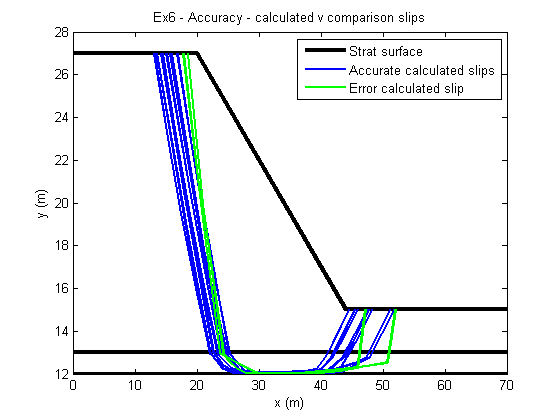
\includegraphics [width=5in]{./VV_SubDocuments/Ex6Tester_01.png}



The next figure shows the progression of the factors of safety through
the generations for each search. The results tend to not show a single
specific path the slips with factors of safety less than 1 take towards
convergence.


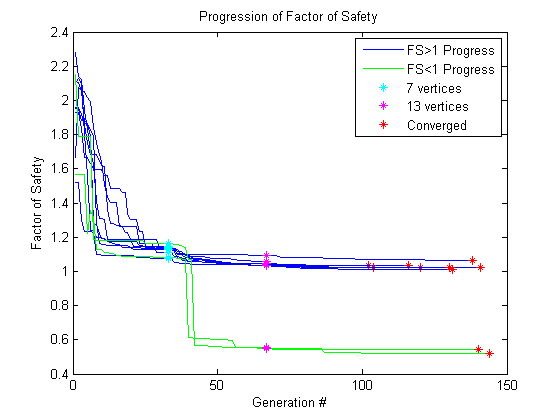
\includegraphics [width=5in]{./VV_SubDocuments/Ex6Tester_02.png}



The next figure of the distribution of factors of safety clearly shows
the bimodal distribution of critical factors of safety generated by the
search.


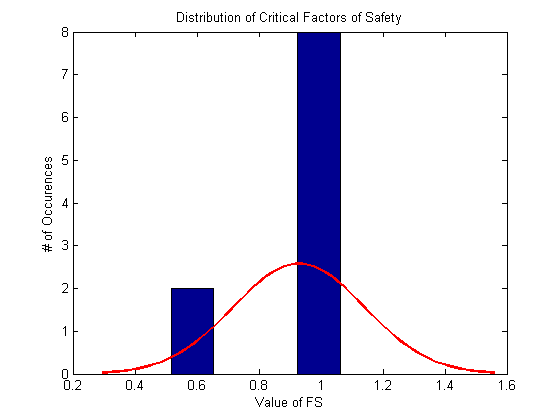
\includegraphics [width=5in]{./VV_SubDocuments/Ex6Tester_03.png}



The genetic algorithm operates by using the Morgenstern Price algorithm
to calculate factors of safety. The factor of safety calculated for the
critical slip by the Morgenstern Price solver is compared to the Rigid
finite element algorithm. Results found in the following table.

        
\color{lightgray} \begin{verbatim}
Type       Morgenstern Price        RFEM    relative error
Accurate        1.0217            1.1683      14.3456
Accurate        1.0345            1.2078      16.7444
Accurate        1.0617            1.1922      12.2930
Accurate        1.0205            1.1641      14.0712
Accurate        1.0353            1.1929      15.2284
Accurate        1.0209            1.1672      14.3306
Accurate        1.0097            1.1520      14.0884
Accurate        1.0248            1.1572      12.9240
Error           0.5428            1.3583      150.2475
Error           0.5173            1.3861      167.9533

\end{verbatim} \color{black}
    

These results show disagreement between the Morgenstern Price and RFEM
algorithms, specifically towards the slip surfaces that produce factors
of safety less than 1 in the Morgenstern Price algorithm. This could
suggest that slip surfaces in with the sharp angles shape seen are
difficult for the Morgenstern Price algorithm to calculate accurately.

Next the sharp angle seen produced by the failure cases is studied by
measuring the angle of the final rise of the slip surfaces. Results in
the table below show that the $FS < 1$ cases have a significantly sharper
exit angle. This continues to suggest that the shape of the failure slips
may be the performance issues.

        
\color{lightgray} \begin{verbatim}
Type        exit angle        Kin Pass    Failure Code
Accurate        2.5570               1          
Accurate        2.4633               1          
Accurate        2.3903               1          
Accurate        2.6349               1          
Accurate        2.4936               1          
Accurate        2.5700               1          
Accurate        2.5328               1          
Accurate        2.4775               1          
Error           2.1022               1           
Error           2.0672               1           

The average rise angle of the slopes with factors of safety
 greater than 1 is 2.515 rads, while the average rise angle 
 of slopes with factors of safety less than 1 is 2.085 rads.
\end{verbatim} \color{black}
    

Using a special test case, where the minimum allowable angle was raised
(to 2.3 rads, 130 deg) the occurrence rate of low factor of safety 
results produced by the genetic algorithm is seen to drop. This could be 
a case that the shape of the failure surface is the performance issue, 
but may also simply be masking a different performance issue. This change
produced no noticeable affect on the results of the other genetic
algorithm calculations performed in \ref{sec:GenAlgTests}. A case could
be made for raising the minimum allowable angle, but a wider range of
test cases would have to be studied before making this decision.





\end{document}
  


